\documentclass[12pt, openright, oneside, a4paper, brazil]{abntex2}
\usepackage[T1]{fontenc}
\usepackage[utf8]{inputenc}
\usepackage{mathptmx}
\usepackage{graphicx}
\usepackage{indentfirst}
\usepackage[expansion=false]{microtype}
\usepackage{url}
\usepackage{hyperref}

\usepackage{ragged2e}

\hypersetup{
  colorlinks = true,
  linkcolor  = black,
  citecolor  = black,
  urlcolor   = blue
}
\makeatletter
\renewcommand{\bibsection}{
  \begingroup
    \let\centering\raggedright
    \chapter*{\bibname}
  \endgroup
  \bibmark
  \ifnobibintoc\else
    \phantomsection
    \addcontentsline{toc}{chapter}{\texorpdfstring{\MakeTextUppercase{\bibname}}{\bibname}}
  \fi
  \prebibhook
}
\makeatother
\addto\captionsbrazil{\renewcommand{\bibname}{REFER\^ENCIAS BIBLIOGR\'AFICAS}}
\makeatletter
\providecommand{\abnt@option@file}{false}
\makeatother
\DeclareOldFontCommand{\tt}{\normalfont\ttfamily}{\mathtt}
\providecommand{\htmladdnormallink}[2]{#1}
\usepackage[alf,abnt-full-initials=yes]{abntex2cite}
\titulo{ANÁLISE E PROPOSTA DE ADEQUAÇÃO DO LABORATÓRIO DE INFORMÁTICA DO CEEP-PMRG}
\autor{ANDRESSA FANTHYNNE GOMES DE ARAÚJO \\ DAVI SAMUEL GREGORIO ALVES \\ FELIPE PELONHA PIMENTEL}
\local{Alto do Rodrigues / RN}
\data{Dezembro / 2022}

\orientador{FRANCISCA LÍGIA DE ARAÚJO}
\coorientador{JOÃO VITOR COSTA CARDOSO}

\instituicao{
  \resizebox{\textwidth}{!}{
    \begin{tabular}{c}
      GOVERNO DO ESTADO DO RIO GRANDE DO NORTE \\
      SECRETARIA DE ESTADO DA EDUCAÇÃO, DA CULTURA, DO ESPORTE E DO LAZER - SEEC \\
      6ª DIREC - DIRETORIA REGIONAL DA EDUCAÇÃO, DA CULTURA E DOS ESPORTES \\
      CENTRO ESTADUAL DE EDUCAÇÃO PROFISSIONAL PROF.ª MARIA RODRIGUES GONÇALVES
    \end{tabular}
  }
}

\preambulo{Artigo apresentado ao Centro Estadual de Educação Profissional Prof.ª Maria Rodrigues Gonçalves, como requisito obrigatório para obtenção do título profissionalizante Técnico em Informática.}
\renewcommand{\imprimircapa}{
  \begin{capa}
    \centering
    
\includegraphics[height=2.50cm, width=3.75cm]{images/CEEP-PMRG_Brank-Mark.png}\par
    \vspace{0.5cm}
    {\ABNTEXchapterfont\bfseries\small\imprimirinstituicao\par}
    
    \vfill
    {\fontsize{14}{16}\selectfont\bfseries \imprimirtitulo\par}
    
    \vfill
    {\fontsize{12}{14}\selectfont \imprimirautor\par}
    
    \vfill
    {\fontsize{12}{14}\selectfont \imprimirlocal\par}
    {\fontsize{12}{14}\selectfont \imprimirdata\par}
    \vspace*{1cm}
  \end{capa}
}
\makeatletter
\renewcommand{\folhaderostocontent}{
  \begin{center}
    {\fontsize{12}{14}\selectfont \imprimirautor\par}
    
    \vspace*{\fill}
    {\fontsize{14}{16}\selectfont\bfseries \imprimirtitulo\par}
    \vspace*{\fill}
    
    \hfill
    \begin{minipage}{0.5\textwidth}
      \begin{SingleSpace}
        \fontsize{10}{12}\selectfont
        \imprimirpreambulo
      \end{SingleSpace}
    \end{minipage}
    
    \vspace*{\fill}
    
    \begin{SingleSpace}
      \fontsize{11}{13}\selectfont
      \rule{8cm}{0.4pt}\par
      \textbf{\imprimirorientador}\par
      Professora Orientadora\par
      \vspace{0.8cm}
      \rule{8cm}{0.4pt}\par
      \textbf{\imprimircoorientador}\par
      Professor Coorientador\par
    \end{SingleSpace}
    
    \vspace*{\fill}
    
    {\fontsize{12}{14}\selectfont \imprimirlocal\par}
    {\fontsize{12}{14}\selectfont \imprimirdata\par}
    \vspace*{1cm}
  \end{center}
}
\makeatother
\renewcommand{\ABNTEXchapterfont}{\fontfamily{ptm}\selectfont\bfseries}
\renewcommand{\ABNTEXchapterfontsize}{\large}

\renewcommand{\ABNTEXsectionfont}{\fontfamily{ptm}\selectfont\bfseries}
\renewcommand{\ABNTEXsectionfontsize}{\normalsize}

\renewcommand{\ABNTEXsubsectionfont}{\fontfamily{ptm}\selectfont\normalfont}
\renewcommand{\ABNTEXsubsectionfontsize}{\normalsize}

\captiontitlefinal{}
\makeatletter
\cftsetindents{chapter}{0pt}{2.5em}
\cftsetindents{section}{1.5em}{3.0em}
\cftsetindents{subsection}{3.0em}{3.5em}
\makeatother
\begin{document}
\imprimircapa
\imprimirfolhaderosto
\newpage
\begin{center}
  {\fontsize{14}{16}\selectfont\bfseries \imprimirtitulo \par}
  \vspace{0.6cm}
  
  {\fontsize{12}{14}\selectfont
    Andressa Fanthynne Gomes de Araújo\textsuperscript{1}, 
    Davi Samuel Gregorio Alves\textsuperscript{1}, 
    Felipe Pelonha Pimentel\textsuperscript{1}\par
    \vspace{0.2cm}
    Francisca Lígia de Araújo\textsuperscript{2}, 
    João Vitor Costa Cardoso\textsuperscript{3}
  }
\end{center}

\vspace{0.8cm}

\begin{center}
  {\bfseries\large RESUMO}
\end{center}

\vspace{0.4cm}

\begin{SingleSpace}
  \noindent
  Este trabalho retrata a importância da adequação e do uso dos laboratórios de informática para as instituições, pois é necessário que estes ambientes estejam bem estruturados de acordo com o que é previsto pelas normas. Desse modo, tem como objetivo produzir uma planta baixa para a adequação do Laboratório de Informática no Centro Estadual de Educação Profissional Professora Maria Rodrigues Gonçalves. Sendo assim, propomos um processo de adequação no espaço, visando à melhoria no rendimento dos alunos na área técnica — que acaba sendo prejudicada pelas condições dispostas no momento, afetando o desempenho dos estudantes. Conclui-se que adequar esse espaço em sua estrutura e organização melhora o interesse dos estudantes da base técnica. Com isso, buscamos trazer mais conforto e praticidade para as aulas, beneficiando tanto os estudantes quanto os profissionais de ensino.
  
  \vspace{0.6cm}
  \noindent\textbf{PALAVRAS-CHAVE:} Laboratório de Informática -- Adequação -- Normas -- Tecnologia.
\end{SingleSpace}

\footnotetext[1]{Alunos concluintes do curso Técnico em Informática, CEEP-PMRG, 2022.}
\footnotetext[2]{Licenciada em Informática, IFRN, 2018; Especialista em Educação e Contemporaniedade, IFRN, 2021; Especialista em Mídias na Educação, UERN, 2022.}
\footnotetext[3]{Licenciado em Computação e Informática, UFERSA, 2021.}
\newpage
\begin{center}
  {\fontsize{14}{16}\selectfont\bfseries Analysis and Adaptation Proposal for the Computer Science Laboratory at CEEP-PMRG \par}
  \vspace{0.6cm}
  
  {\fontsize{12}{14}\selectfont
    Andressa Fanthynne Gomes de Araújo\textsuperscript{1}, 
    Davi Samuel Gregorio Alves\textsuperscript{1}, 
    Felipe Pelonha Pimentel\textsuperscript{1}\par
    \vspace{0.2cm}
    Francisca Lígia de Araújo\textsuperscript{2}, 
    João Vitor Costa Cardoso\textsuperscript{3}
  }
\end{center}

\vspace{0.8cm}

\begin{center}
  {\bfseries\large ABSTRACT}
\end{center}

\vspace{0.4cm}

\begin{SingleSpace}
  \noindent
  This work portrays the importance of proper adequacy and utilization of computer labs in institutions, as these environments must be well structured according to established standards. Therefore, it aims to design a floor plan for the Computer Laboratory at the State Center for Professional Education Professor Maria Rodrigues Gonçalves. We propose an adaptation process for the lab to improve the performance of technical students, which is currently hindered by existing conditions. It is concluded that updating the structure and organization of this space enhances student engagement in technical courses, creating a more comfortable and practical environment for both students and teaching professionals.
  
  \vspace{0.6cm}
  \noindent\textbf{KEYWORDS:} Computer Lab -- Adequacy -- Standards -- Technology.
\end{SingleSpace}

\footnotetext[1]{Alunos concluintes do curso Técnico em Informática, CEEP-PMRG, 2022.}
\footnotetext[2]{Licenciada em Informática, IFRN, 2018; Especialista em Educação e Contemporaniedade, IFRN, 2021; Especialista em Mídias na Educação, UERN, 2022.}
\footnotetext[3]{Licenciado em Computação e Informática, UFERSA, 2021.}
\newpage
\pdfbookmark[0]{\listfigurename}{lof}
\listoffigures*
\cleardoublepage
\newpage
\pdfbookmark[0]{Lista de abreviaturas e siglas}{lsf}
\begin{siglas}
  \item[BTU] \textit{British Thermal Unit} (Unidade Térmica Britânica)
  \item[CEEP-PMRG] Centro Estadual de Educação Profissional Professora Maria Rodrigues Gonçalves
  \item[FNDE] Fundo Nacional de Desenvolvimento da Educação
  \item[MEC] Ministério da Educação
  \item[ProInfo] Programa Nacional de Tecnologia Educacional
  \item[QDF] Quadro de Distribuição de Força
  \item[RN] Rio Grande do Norte
  \item[TICs] Tecnologias de Informação e Comunicação
  \item[UTP] \textit{Unshielded Twisted Pair} (Par Trançado Não Blindado)
\end{siglas}
\cleardoublepage
\newpage
\thispagestyle{empty}
\pdfbookmark[0]{\contentsname}{toc}
\begin{center}
  {\bfseries\large SUMÁRIO}
\end{center}
\vspace{0.6cm}

\begingroup
  \makeatletter
  \renewcommand{\printtoctitle}[1]{}
  \makeatother
  
  \tableofcontents*
\endgroup

\cleardoublepage

\newpage
\pagestyle{simple}
\textual

\chapter{INTRODUÇÃO}
	A utilização de laboratórios de informática nas escolas estaduais do Rio Grande do Norte (RN) tem sido de suma importância para o ensino e a aprendizagem de estudantes das escolas técnicas, pois contribui significativamente para a sua formação acadêmica mediante os conhecimentos adquiridos através das tecnologias implementadas nas instituições de ensino.

	Em vista disso, o Ministério da Educação (MEC), em parceria com os governos estaduais e municipais, promoveu a implementação e o uso dessas tecnologias — a exemplo do laboratório de informática — por meio do Programa Nacional de Tecnologia Educacional (ProInfo Integrado) nas instituições de ensino \cite{lobler2012renote}.

	Sendo assim, busca-se resposta para a seguinte problemática: como a correta adequação do Laboratório de Informática na instituição escolar CEEP-PMRG pode melhorar o ensino e a aprendizagem, visando compreender a estrutura, a implementação e a utilização deste ambiente?

	Com isso em mente, este trabalho aponta a importância da adequação do Laboratório de Informática da instituição escolar CEEP-PMRG como fonte de melhoria no processo de aprendizagem dos estudantes da base técnica de ensino. Desse modo, teve como objetivo geral produzir uma planta baixa para a adequação do Laboratório de Informática no Centro Estadual de Educação Profissional Professora Maria Rodrigues Gonçalves (CEEP-PMRG). Como objetivos específicos: 1. Contextualizar o processo de implementação dos Laboratórios de Informática nas instituições de ensino do Rio Grande do Norte; 2. Identificar os pontos de atenção presentes na infraestrutura do Laboratório de Informática do CEEP-PMRG; e 3. Propor soluções para os problemas identificados no Laboratório de Informática, por meio de uma planta baixa desenvolvida de acordo com a avaliação do projeto da própria escola e a análise dos pesquisadores.

	O interesse e a motivação para a realização desta pesquisa surgiram do intuito de verificar as perspectivas de adequação do Laboratório de Informática. Com base na realidade atual, foram efetuadas observações atento-se aos pontos presentes na infraestrutura — diante das pesquisas realizadas e conforme o que é recomendado — para melhorias e acompanhamento das aulas.

	Conclui-se que os Laboratórios de Informática devem estar presentes não apenas nas escolas técnicas, mas também em todas as instituições de ensino, em especial nas escolas públicas. A presença destes ambientes contribui para o aprimoramento tanto do ensino por parte dos docentes quanto do aprendizado por parte dos discentes. Porém, para que essa ideia saia do papel e se torne uma realidade, é necessário que os laboratórios tenham uma boa infraestrutura, oferecendo conforto e segurança aos que deles se beneficiam, encaixando-se, assim, nos padrões exigidos.

	Desse modo, este trabalho estrutura-se da seguinte forma: 1. Introdução, tópico que aborda a relevância do trabalho desenvolvido, bem como os objetivos almejados. No 2. Referencial Teórico, abordamos a seção 2.1 Laboratórios de Informática Aliados à Aprendizagem, que apresenta a relevância desse espaço nas instituições escolares. Trata-se também da 2.2 Estrutura do Laboratório de Informática CEEP-PMRG, destacando as normas técnicas e éticas que envolvem a organização, a distribuição das instalações elétricas, dos computadores e da mobília, entre outros aspectos. Na 3. Metodologia, constam os métodos utilizados para a construção e a análise do trabalho (onde se realizou uma análise cuidadosa sobre o laboratório da escola-campo da pesquisa, demonstrando elementos que precisam de atenção embasada por normas). Nos 4. Resultados e Discussões, descrevemos os pontos analisados do Laboratório de Informática a fim de propor soluções. Por fim, nas Considerações Finais, discorre-se sobre os resultados alcançados e o desfecho do trabalho, tratando dos pontos principais e da relevância do tema para o ensino e a aprendizagem.
\newpage
\chapter{REFERENCIAL TEÓRICO}
\section{LABORATÓRIOS DE INFORMÁTICA ALIADOS À APRENDIZAGEM}

	Os Laboratórios de Informática estão cada vez mais presentes nos projetos de desenvolvimento das escolas, visto que a sua utilização é um recurso de grande relevância para o ensino e a aprendizagem — afinal, a informatização é uma realidade no dia a dia da sociedade e, portanto, deve estar integrada às instituições de ensino.

	Contudo, é importante atentar-se aos déficits presentes em algumas destas instituições, os quais podem afetar a estrutura desse ambiente e, por consequência, impactar as ações de docentes e estudantes. De acordo com \citeonline{silva2015}, algumas instituições deixam de oferecer laboratórios ou profissionais capacitados na área de informática, fazendo com que os alunos sofram prejuízos no nível de aprendizagem. Sendo assim, compreende-se que a falta de adequação dos laboratórios pode ocasionar forte impacto na produtividade dos alunos.

\begin{citacao}
	Acredita-se que professores e alunos ao encontrarem laboratórios bem cuidados, tanto na parte predial, como de hardware e software, terão mais disposição, interesse e ganho de produtividade nas atividades a serem desenvolvidas. Um ambiente agradável, limpo e organizado, com equipamentos e programas de computador funcionando bem, torna tudo mais interessante, e os usuários terão confiança naquilo que utilizam. \cite[p.~22]{gripa2002}
\end{citacao}

	Ainda em consonância com os autores, é fundamental que os laboratórios sejam bem organizados e estruturados para permitir a execução eficiente do planejamento de professores de diferentes áreas — e, em especial, das práticas previstas nas grades curriculares de alunos dos cursos técnicos da área de informática. Essa estruturação influencia positivamente o desempenho dos trabalhos e das pesquisas realizadas pelos estudantes, proporcionando-lhes conforto e agilidade.

	Sendo assim, compreendemos que formar profissionais capacitados para o mundo do trabalho exige mais do que a abordagem de conteúdos; requer atenção ao modo como estes são mediados pelos professores. Portanto, os laboratórios de informática influenciam a aprendizagem significativa dos discentes, bem como o seu desenvolvimento técnico.

	Aliado a isso, destaca-se que as Tecnologias de Informação e Comunicação (TICs) podem proporcionar a ampliação das práticas de ensino direcionadas à aprendizagem. De acordo com \citeonline[p.~70]{nobre2015}:

\begin{citacao}
		O computador associado a outros recursos de TICs se transforma em uma ferramenta com alta potencialidade para apoiar o desenvolvimento do processo de ensino-aprendizagem dos alunos. Não se trata apenas de saber manusear tal recurso, mas de focar o objetivo do uso deste em situações que promovam a construção do conhecimento.
\end{citacao}

	Sendo assim, quando essas tecnologias são associadas ao uso dos laboratórios de informática, podem potencializar o ensino e a aprendizagem de estudantes e professores, incentivando, inclusive, o interesse dos alunos pelo conteúdo ministrado.

O acesso ao ambiente também deve ser considerado para o bom uso desse espaço. A utilização, a organização e a manutenção dos equipamentos são partes importantes da estrutura dos laboratórios e, nesse sentido, é essencial que o acesso de pessoas ao local seja organizado. Segundo \citeonline{nobre2015} as escolas podem trabalhar de forma sistematizada e não sistematizada. A sistematizada refere-se à definição de horários para o acesso de professores e alunos ao laboratório de informática — isto é, os horários de cada professor já estão estipulados no planejamento elaborado pelo coordenador pedagógico —, enquanto a não sistematizada está relacionada ao interesse do professor em ter acesso ao laboratório, sem imposição de uso, ficando o docente livre para utilizar o espaço de acordo com suas necessidades pedagógicas.

Portanto, embora as especificações técnicas sejam de suma importância para este ambiente, é preciso pensar também em como os equipamentos da sala poderão ser preservados de modo a evitar a avaria dos computadores, dos dispositivos de rede e das instalações existentes. Para isso, apresenta-se a seguir como deve ser a estrutura do ambiente, bem como a ética relacionada à sua utilização.

\section{ESTRUTURA DO LABORATÓRIO DE INFORMÁTICA}

	Para construir uma visão geral da estrutura de um Laboratório de Informática, utilizou-se como referência a cartilha do Programa Nacional de Tecnologia Educacional — \citeonline{proinfo2009}, que faz as recomendações para a montagem de laboratórios de informática na escola, além de outros autores que contribuíram para a discussão.

Compreender o espaço disponível para as salas de informática é parte importante do processo de organização e estrutura. Segundo recomendações do \citeonline{proinfo2009} deve haver uma distribuição adequada dos computadores considerando a quantidade de alunos, sendo recomendado um estudante por máquina para garantir um ambiente adequado à aprendizagem. Dessa forma, a distribuição "[...] deverá contemplar, no mínimo, 2m² para cada computador a ser instalado, de forma a garantir um mínimo de espaço para a operação dos equipamentos pelos respectivos alunos, provendo um ambiente de aprendizagem agradável e confortável."

	Quanto ao {\textit layout} (organização) do ambiente, segundo \citeonline{gripa2002}, a disposição ou o posicionamento de cada equipamento pode ser feito em formato de fileiras, sendo este o método mais tradicional. Nesse sentido, é preciso considerar que o espaço deve comportar, além dos equipamentos, a mobília adequada, pois, ainda de acordo com o autor, "os ambientes devem ser projetados para ter-se um bom aproveitamento do espaço físico e dos equipamentos, bem como oferecer o máximo de conforto aos usuários" \cite[p.~114]{gripa2002}.

	Além disso, a infraestrutura do laboratório de informática deve ser protegida contra agentes agressivos, tais como areia, poeira ou chuva, além de estar distante de tubulações hidráulicas para garantir a integridade dos equipamentos instalados, de modo que tais agentes não venham a danificar os computadores nem provocar desconforto aos alunos e aos demais ocupantes \cite{proinfo2009}.

	Outro detalhe ao qual se deve atentar e que é de extrema importância refere-se ao espaço onde o laboratório de informática funcionará, pois jamais deve estar localizado próximo à umidade (como banheiros) ou a locais com muita poeira, calor, odor e barulho \citeonline{gripa2002}. Recomenda-se a adequação do piso, que não deve possuir desníveis que possam provocar a queda de ocupantes ou o acúmulo de resíduos e água. Exemplos adequados são os pisos de cimento liso, pedra ou cerâmica, desde que não gerem energia estática pelo atrito com os calçados, descartando a possibilidade de descargas elétricas que atinjam e danifiquem os equipamentos.

Além disso, a temperatura do ambiente também deve ser levada em consideração, já que, de acordo com o documento do \citeonline[p.~5]{proinfo2009}:

\begin{citacao}
		{[\dots]} a temperatura ambiente deve ser de no máximo 30°C. Se não for possível em condições naturais, deverá ser instalado um aparelho de ar-condicionado de, no mínino, 18.000 BTU. As especificações técnicas de temperatura para o perfeito funcionamento do laboratório e de equipamentos de informática não podem ser altas, pois correm o risco de danificar as máquinas, além de ser desconfortável para os alunos.
\end{citacao}

	Mais um elemento que não pode ser deixado de lado é a instalação elétrica dos laboratórios de informática, pois existem diversos elementos que devem ser implementados para a utilização dos computadores e demais aparelhos. A falta de adequação dessa instalação pode ser um fator crítico para o bom funcionamento dos equipamentos e para a segurança dos usuários. Conforme \citeonline[p.~119]{gripa2002}:

\begin{citacao}
		Cada laboratório deverá dispor de um quadro de distribuição de energia elétrica. Dotado de um aterramento real feito por malha e barras de cobre enterradas no chão, com resistência final menor que $10\,\Omega$, medida por equipamento específico. Este quadro de distribuição exclusivo para os computadores, deverá conter disjuntores de proteção. O consumo estimado de um microcomputador é de cerca de 600 watts.
\end{citacao}

	Nesses ambientes, é comum utilizar tomadas, porém elas não devem ser compartilhadas com a rede elétrica de iluminação, pois interferências podem ser geradas por outros aparelhos. Dessa forma, os tipos de tomadas recomendados são as monofásicas de 3 (três) pinos, padrão NEMA 5P, instaladas ao longo das paredes, em caixas modulares externas ou embutidas — uma para cada equipamento (microcomputador, impressora, {\textit hub} e {textit scanner}, se houver).

	Diante das especificações técnicas necessárias para estruturar o ambiente de um Laboratório de Informática, é possível fazer uma análise desse espaço no CEEP-PMRG, no município de Alto do Rodrigues/RN, que apresenta condições limitadas quanto à sua estrutura, podendo causar impactos negativos nos métodos dos professores e na aprendizagem dos estudantes.


\chapter{ANÁLISE DO LABORATÓRIO DE INFORMÁTICA CEEP-PMRG}

	Como anunciado na introdução deste trabalho, a análise foi realizada na escola profissionalizante CEEP-PMRG, localizada no município de Alto do Rodrigues/RN, a qual possui diversos laboratórios de diferentes áreas do conhecimento. Reconhecidamente, é um centro que visa à formação técnica nas áreas de Energias Renováveis e de Informática — sendo esta última o foco do trabalho. Sendo assim, o espaço analisado dentre os laboratórios foi o de Informática, que atende aos estudantes da instituição, mais especificamente os alunos do curso Técnico em Informática. Desse modo, a partir da planta baixa deste espaço, foi possível fazer um comparativo entre o planejamento do ambiente e suas especificações técnicas e o que se apresenta na realidade dos estudantes. A imagem aponta para as especificações técnicas, o planejamento do espaço, a organização e a implementação.

\begin{figure}[htb]
	\centering
	\caption{Planta Baixa Real - Lab. Infor. CEEP-PMRG}
	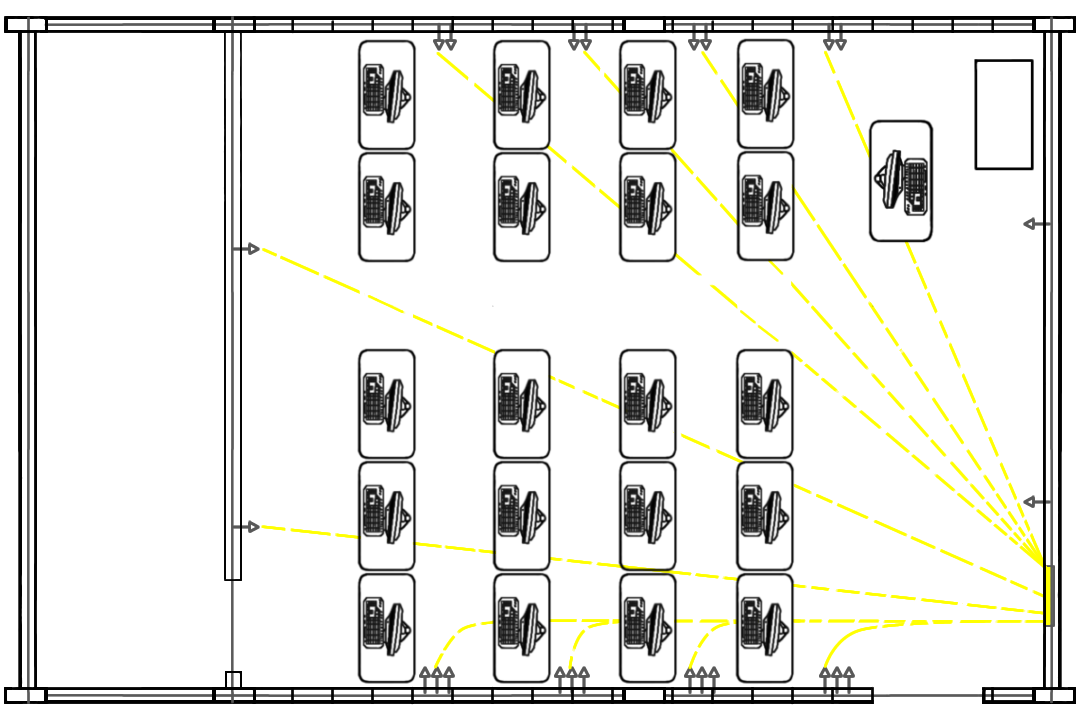
\includegraphics[width=0.80\textwidth]{figures/figura-01_planta-lab.png}
	\legend{Fonte: Autoria Própria (2022)}
	\label{fig:01_planta-baixa}
\end{figure}

	É possível perceber que a quantidade ideal de computadores suportada pelo espaço (que mede 7 metros de largura por 10 metros de comprimento) é de 21 máquinas, fazendo-se uso do mobiliário adequado. O que se nota, no entanto, é que o espaço não comporta adequadamente os 30 computadores atuais e o mobiliário não é adequado, já que são usadas carteiras das salas de aula para acomodar as máquinas, tornando o espaço entre elas ainda mais limitado. Isso causa problemas, inclusive, com a organização dos cabos de alimentação e periféricos (como mouse e teclado), dificultando o manuseio dos acessórios.
\clearpage

	Dada a forma como os 30 computadores estão distribuídos no espaço do Laboratório de Informática — com fileiras separadas por distâncias inferiores ao padrão estabelecido, que "[...] deverá contemplar, no mínimo, 2 m² para cada computador a ser instalado" \cite{proinfo2009} —, decorrem alguns problemas. As distribuições dos cabos de energia e de conexão de vídeo se entrelaçam e, por vezes, se desprendem dos dispositivos, ocasionando o desligamento das máquinas. A locomoção do professor para orientar os alunos durante as atividades também é prejudicada pelo pouco espaço entre os computadores. Com a proximidade das máquinas entre as fileiras, a visualização do conteúdo projetado no quadro pode ser inviabilizada em virtude da posição dos monitores.

	A temperatura desse ambiente conta com uma climatização por meio de um ar-condicionado de 35.000 BTUs (British Thermal Unit ou Unidade Térmica Britânica), atendendo às especificações recomendadas pelo ProInfo (1997). Em relação aos cuidados, são necessárias manutenções frequentes no equipamento para que não ocorram gotejamentos de água sobre o ambiente, o que geraria o risco de atingir as tomadas ou computadores e provocar a queima dos equipamentos. É importante ressaltar também a iluminação: as janelas precisam de cortinas para que a claridade do sol não prejudique os equipamentos e a infraestrutura. O laboratório conta com cortinas escuras, mas a luz solar ainda as ultrapassa por as janelas não serem totalmente adequadas, o que pode ocasionar reflexos no monitor e desviar o foco durante o uso.

	Em relação à quantidade de tomadas instaladas no Laboratório de Informática de acordo com a planta baixa, há 24 tomadas que pertencem ao Quadro de Distribuição de Força (QDF). O QDF é um painel responsável pela distribuição de energia da instituição, proporcionando controle e segurança ao sistema. Conforme o documento do \citeonline[p.~7]{proinfo2009}, para seguir as exigências mínimas da instalação elétrica do ambiente, recomenda-se que:

\begin{citacao}
		{[\dots]} fornecimento de energia elétrica de 110V ou 220V, com capacidade de pelo menos 10 KVA, sendo estes parâmetros o mínimo de carga na rede elétrica para o funcionamento dos equipamentos a serem instalados. Tais como requisitos, se não cumpridos, poderão acarretar na queima de componentes, estabilizadores e dos microcomputadores, em função de possíveis quedas e oscilações inesperadas de energia no laboratório.
\end{citacao}

	A partir da análise da planta baixa do Laboratório de Informática da instituição, constata-se que este possui um QDF com tensão de alimentação — componente capaz de exercer pressão no circuito elétrico para impulsionar a corrente através de um circuito condutor —, permitindo o funcionamento adequado na tensão de alimentação do laboratório (equivalente a 380-220 V, com fator de potência de 92%).

	O Laboratório de Informática do CEEP-PMRG conta com 19 tomadas disponíveis para 30 computadores. Segundo a norma, que exige "tomadas tremulares monofásicas de 3 (três) pinos, padrão NEMA 5P, instaladas ao longo das paredes, em caixas modulares externas ou embutidas, uma para cada equipamento [...]"~\citeonline[p.~9]{proinfo2009}, esse número é insuficiente, dificultando a inclusão de mais máquinas. Para comportar uma quantidade de computadores superior ao número de tomadas, adota-se o uso de estabilizadores. Porém, essa prática ocasiona uma má distribuição dos fios, dificultando a locomoção de professores e alunos no espaço entre as mesas. Quanto às conexões de rede via cabo, o número de entradas RJ-45 também é insuficiente em relação ao número de computadores, inviabilizando o acesso de algumas máquinas à internet e dificultando atividades que demandam conectividade.

	O acesso a esse ambiente prioriza os professores da base técnica em informática, visto que o curso possui maior afinidade e contato com os computadores.

	Para despertar o interesse dos alunos pelo aprendizado, é necessário utilizar metodologias de ensino que envolvam a tecnologia — a exemplo das práticas realizadas no Laboratório de Informática, como a criação de códigos para sites com o uso das linguagens HTML, CSS, JavaScript, PHP e SQL (relacionando o desenvolvimento {\textit web} a bancos de dados), entre outras atividades do currículo do curso.

	Quanto à estrutura de rede do Laboratório de Informática, a Direção disponibilizou como referência o documento do Projeto de Rede Brasil Profissionalizante, elaborado por Carlos Eduardo e Frederico Augusto (Natal/RN, 2009) sob o respaldo do Ministério da Educação e do Fundo Nacional de Desenvolvimento da Educação (FNDE).

	De acordo com o documento, a implementação das caixas de passagem serve para facilitar a passagem do cabeamento {\textit backdone}, distribuído por meio de dutos para dar acesso à rede no ambiente. A ligação da caixa de passagem do laboratório conecta-se ao {\textit rack} 8U e os conectores são do tipo RJ-45, distribuídos por pares trançados, de acordo com a norma EIA/TIA T568. Os cabos são do tipo UTP (\textit{Unshielded Twisted Pair}) ou Par Trançado Não Blindado) sólido de 4 pares, padrão 1000Base-T (1000 Mbps), os quais estão em quantidade inferior ao número de máquinas.

	Tendo como base esses padrões, percebe-se que o Laboratório de Informática possui uma deficiência na infraestrutura de rede, já que a conexão com a internet não funciona em sua plenitude: tanto a rede cabeada quanto a rede {\textit wireless} encontram-se inadequadas aos propósitos de aprendizagem estabelecidos pela instituição. Em virtude disso, evidencia-se a importância de cumprir as especificações técnicas de rede para que o ambiente funcione adequadamente e dentro de todas as normas estabelecidas. estabelecidas.

\chapter{METODOLOGIA}

	A abordagem de pesquisa para a construção do presente trabalho é qualitativa, pois busca compreender a importância da correta adequação do laboratório como recurso mediador da aprendizagem no curso Técnico em Informática. A pesquisa pode ser classificada quanto aos seus objetivos como descritiva e explicativa. É descritiva por abordar uma série de informações levantadas através do método de pesquisa bibliográfica — selecionando artigos e monografias que trazem ideias construtivas para embasar o tema de forma seletiva e analítica — e explicativa por defender a hipótese de que a adequação estrutural desse ambiente pode influenciar o ensino e a aprendizagem de maneira positiva (caso esteja de acordo com as recomendações técnicas) ou negativa.

	Quanto aos procedimentos, o método empregado caracteriza-se como um estudo de caso e diagnóstico estrutural, que busca compreender a realidade enfrentada no Laboratório de Informática do CEEP-PMRG. Utiliza-se a análise sobre a variável de adequação física e tecnológica para testar a hipótese apresentada, propondo a elaboração de uma planta baixa ajustada à realidade da escola com o intuito de sugerir melhorias para o ensino.

	A instituição escolar CEEP-PMRG, localizada no município de Alto do Rodrigues/RN, possui um Laboratório de Informática cuja estrutura, organização e uso contribuem de forma positiva para o ensino-aprendizagem quando utilizado adequadamente. Embora o prédio atenda aos cursos técnicos profissionalizantes de Energias Renováveis e de Informática, a prioridade de uso do espaço é dada aos professores da base técnica em informática, a fim de viabilizar aulas práticas. As condições desse ambiente são favoráveis ao uso; contudo, a adequação física não foi planejada de forma ideal — o que se evidencia na insuficiência de computadores para todos os estudantes e na falta de instalações elétricas para a inclusão de novas máquinas, visando à meta de um computador por aluno. Dessa forma, foi desenvolvida uma planta baixa que projeta a adequação ideal desse Laboratório de Informática.

\chapter{RESULTADOS E DISCUSSÕES}

	A partir das necessidades técnicas e educacionais do Laboratório de Informática do CEEP-PMRG, propõe-se uma estrutura de organização para este ambiente de acordo com as normas técnicas baseadas no \citeonline{proinfo2009}, acompanhada de uma planta baixa que projeta tal adequação a fim de sugerir melhorias ao espaço. Sendo assim, a Figura~\ref{fig:02_planta-baixa-adequada} representa a proposta elaborada conforme as demandas do ambiente, visando a promover um processo de ensino e aprendizagem mais significativo.
\begin{figure}[htb]
	\centering
	\caption{Planta Baixa Adequada - Lab. Infor. CEEP-PMRG}
	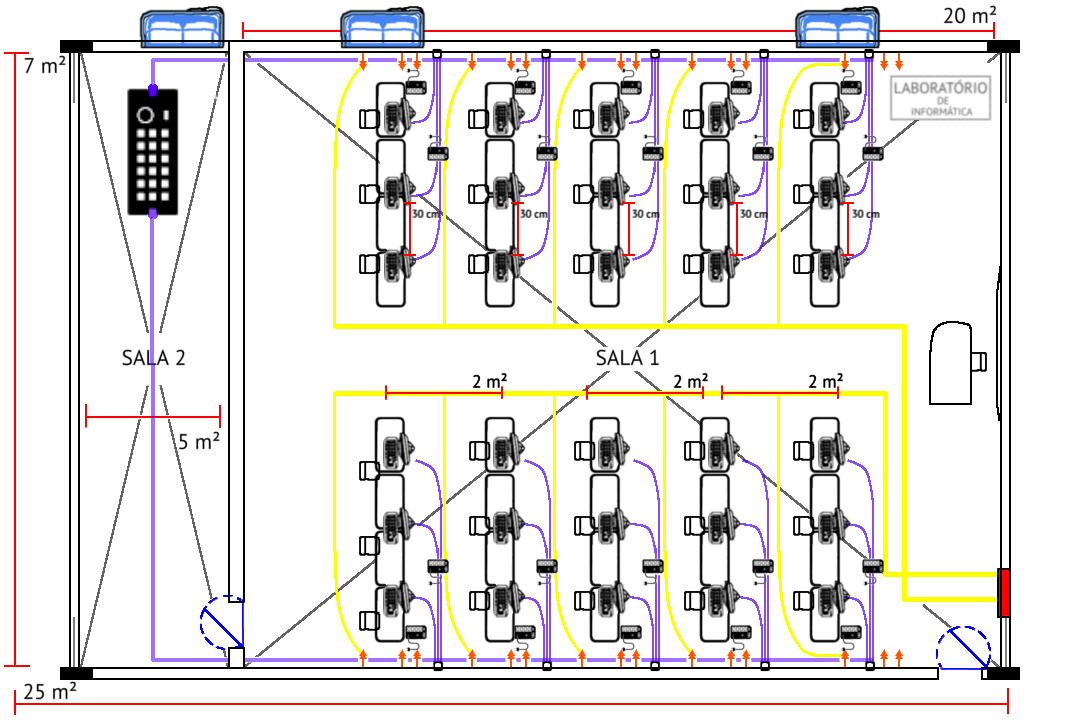
\includegraphics[width=0.95\textwidth]{figures/figura-02_planta-lab-adequada-prop.png}
	\legend{Fonte: Autoria Própria (2022)}
	\label{fig:02_planta-baixa-adequada}
\end{figure}
A imagem apresentada indica a adequação do Laboratório de Informática proposta neste trabalho. Os itens contemplados na planta baixa compreendem: o espaço físico do ambiente, o mobiliário, a distribuição das instalações elétricas e a distribuição dos conectores RJ-45 e cabos UTP da rede. As especificações do projeto abrangem desde a organização e o planejamento do espaço até as normas éticas de uso, a fim de permitir o bom aproveitamento do ambiente e gerar resultados positivos na aprendizagem — contribuindo, assim, para a formação dos estudantes do curso Técnico em Informática do CEEP-PMRG.
\clearpage
\section{ZONA DO AMBIENTE}

	O dimensionamento do espaço em um Laboratório de Informática mostra-se fundamental na forma como as mesas e os computadores são dispostos. Com isso em mente, o local deve ser bem planejado para atender às necessidades de circulação e permitir que a adequação ocorra de forma funcional durante as atividades. A Figura~\ref{fig:03_planta-baixa-adequada-prop-espaco} projeta as duas salas que constituem o Laboratório de Informática do CEEP-PMRG com as devidas medidas propostas.

\begin{figure}[htb]
	\centering
	\caption{Planta Baixa Espaço Adequado - Lab. Infor. CEEP-PMRG}
	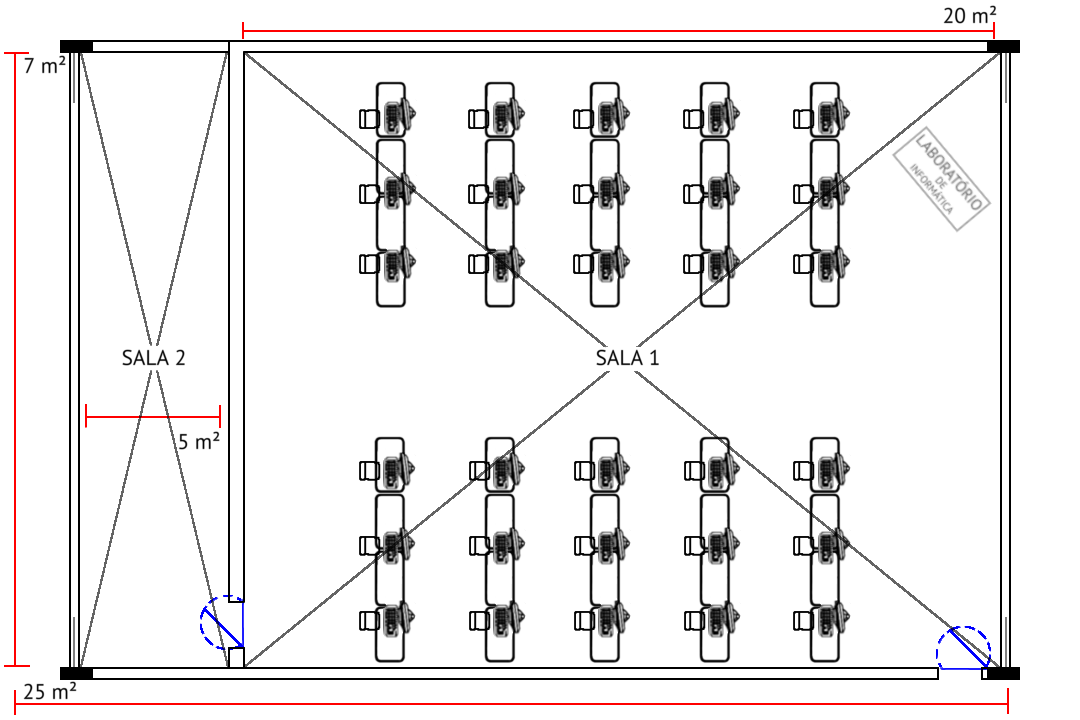
\includegraphics[width=0.90\textwidth]{figures/figura-03_planta-lab-adequada-prop-espaco.png}
	\legend{Fonte: Autoria Própria (2022)}
	\label{fig:03_planta-baixa-adequada-prop-espaco}
\end{figure}

	Constata-se que o espaço atual da sala mede 7 m de largura por 10 m de comprimento, onde os computadores e as mesas estão dispostos. A configuração vigente gera dificuldades decorrentes da falta de espaço entre as fileiras de computadores, o que prejudica a locomoção de professores e estudantes.

	Com o intuito de otimizar o espaço para a organização dos computadores e do mobiliário (mesas e cadeiras), as medidas propostas na Figura~\ref{fig:03_planta-baixa-adequada-prop-espaco} — de 25 metros de comprimento por 7 metros de largura — resolveriam o problema identificado, pois facilitariam a circulação do professor no momento de prestar auxílio aos estudantes durante as aulas.
\clearpage
\section{MOBILIÁRIO E ESPAÇAMENTO}

	Em contraponto à realidade vivenciada, o mobiliário deve ser apropriado para acomodar os computadores, sendo essencial dimensionar a quantidade ideal de bancadas em função do fluxo de alunos.

	O mobiliário deve oferecer, assim como os corredores entre as fileiras, espaço adequado para o manuseio do mouse e uma distância razoável entre os usuários, visto que os estudantes necessitam desse suporte para utilizar outros materiais, como cadernos e canetas. A Figura~\ref{fig:04_planta-lab-adequada-prop-esp-computador} projeta o espaçamento ideal entre os computadores e o arranjo das mesas, apresentando uma área funcional para o desenvolvimento das atividades.

\begin{figure}[htb]
	\centering
	\caption{Planta Baixa Adequado Espaçamento Computadores - Lab. de Infor. CEEP-PMRG}
	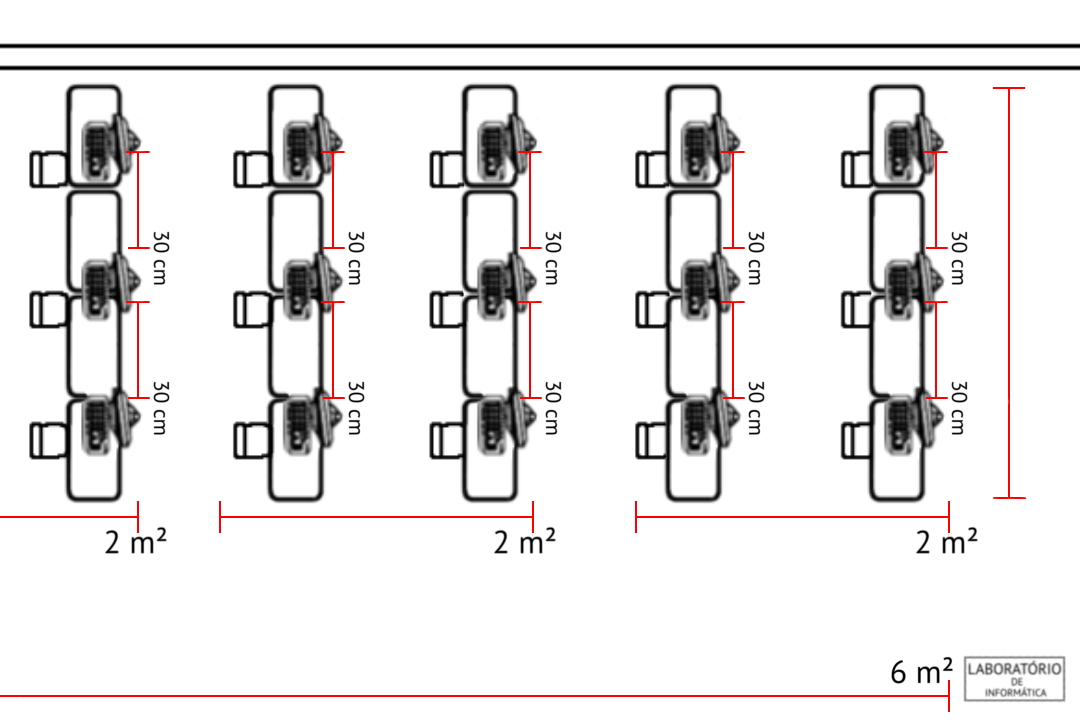
\includegraphics[width=0.80\textwidth]{figures/figura-04_planta-lab-adequada-prop-esp-computador.png}
	\legend{Fonte: Autoria Própria (2022)}
	\label{fig:04_planta-lab-adequada-prop-esp-computador}
\end{figure}

	Compreende-se que dispor quatro mesas por fileira garante um espaço significativo para o manuseio dos periféricos (como mouse e teclado), além de permitir o espaçamento adequado entre as máquinas, proporcionando maior conforto aos estudantes. Ademais, planejar esse espaçamento é uma medida de inclusão, pois viabiliza a acessibilidade de pessoas com mobilidade reduzida, como usuários de cadeira de rodas.

	Quanto aos cabos que atualmente encontram-se espalhados pelo chão, deve haver a sua devida organização: eles devem ser agrupados e fixados sob as mesas para evitar acidentes.
\clearpage
\section{DISTRIBUIÇÃO DAS TOMADAS}

	Em relação às instalações elétricas, para atender à quantidade de computadores existentes no Laboratório de Informática, as tomadas devem ser do tipo monofásicas de 3 (três) pinos, padrão NEMA 5P (conforme a norma). Atualmente, o laboratório conta com 17 tomadas, número que não supre a demanda de equipamentos devido tanto à quantidade insuficiente quanto à disposição do espaço. A Figura~\ref{fig:05_planta-lab-adequada-prop-dist-eletrica} demonstra um comparativo de como os estabilizadores poderiam se adequar ao ambiente.

\begin{figure}[htb]
	\centering
	\caption{Planta Baixa Adequada Distribuição Elétrica - Lab. Infor. CEEP-PMRG}
	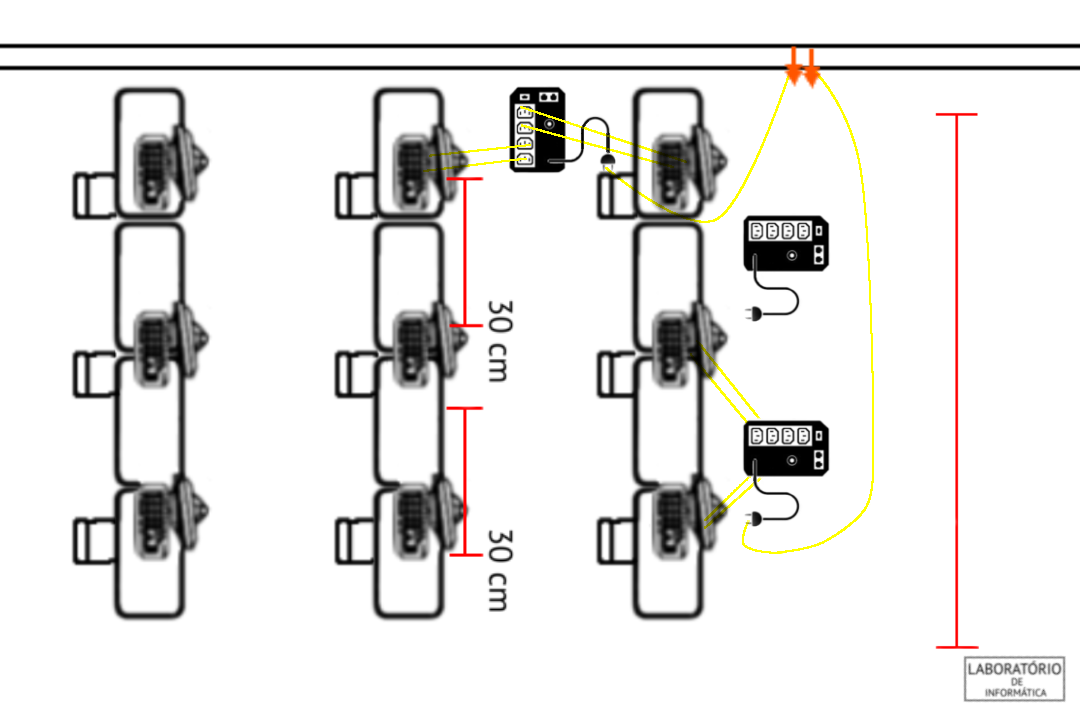
\includegraphics[width=0.75\textwidth]{figures/figura-05_planta-lab-adequada-prop-dist-eletrica.png}
	\legend{Fonte: Autoria Própria (2022)}
	\label{fig:05_planta-lab-adequada-prop-dist-eletrica}
\end{figure}

	A distribuição dos estabilizadores no Laboratório de Informática deve ser quantitativamente adequada e apresentar especificações técnicas compatíveis com a voltagem das tomadas e dos conectores (no exemplo citado, os estabilizadores possuem quatro tomadas de 3 pinos). Esses dispositivos são necessários para manter maior número de computadores em funcionamento simultâneo enquanto o total de tomadas de parede for inferior ao de máquinas.
\clearpage
\section{CONECTORES RJ-45 E CABOS UTP}

	Como mencionado anteriormente, a Sala 02 do Laboratório de Informática do Centro Estadual de Educação Profissional Professora Maria Rodrigues Gonçalves possui um {\textit rack} 8U responsável por distribuir o sinal de internet via cabeamento estruturado, conforme ilustrado na Figura~\ref{fig:06_planta-lab-adequada-prop-dist-rede}.

\begin{figure}[htb]
	\centering
	\caption{Planta Baixa Adequada Distribuição Rede - Lab. Infor. CEEP-PMRG}
	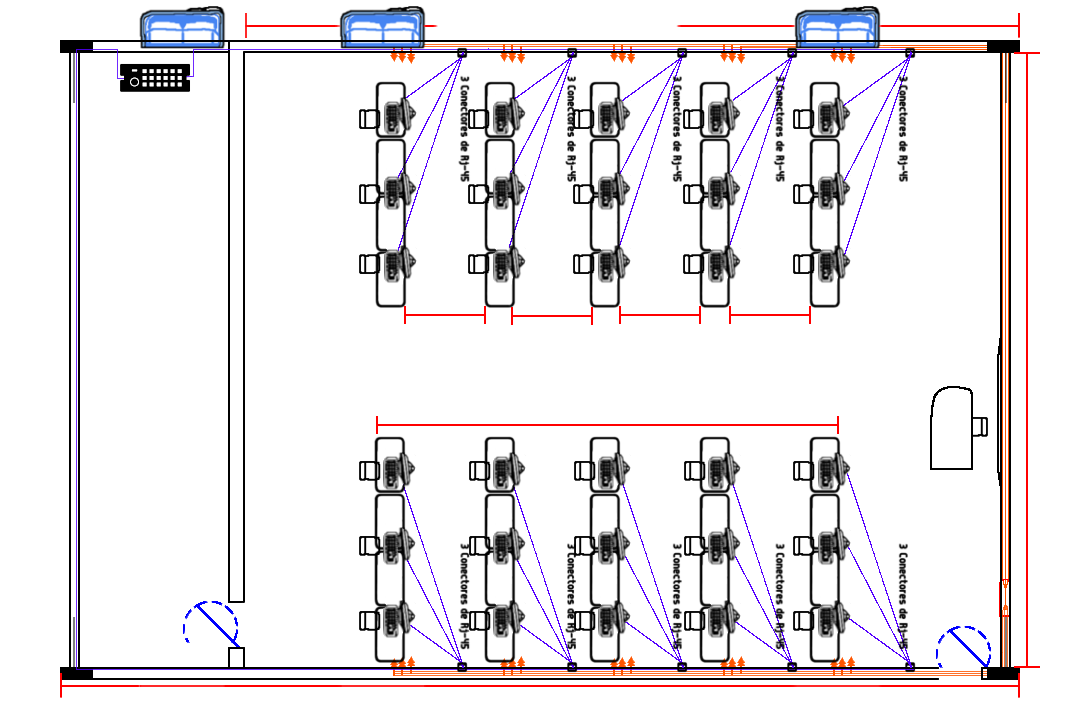
\includegraphics[width=0.85\textwidth]{figures/figura-06_planta-lab-adequada-prop-dist-rede.png}
	\legend{Fonte: Autoria Própria (2022)}
	\label{fig:06_planta-lab-adequada-prop-dist-rede}
\end{figure}

	Atualmente, há cerca de 30 conectores RJ-45 duplos, dos quais alguns se encontram inoperantes. Desse modo, faz-se necessária a substituição desses componentes e a adequação da infraestrutura de cabeamento, visando à melhoria da rede de internet do laboratório, visto que a conexão cabeada oferece maior estabilidade de uso.
	A partir do exposto, compreende-se que as melhorias sugeridas neste trabalho são de suma importância para readequar o ambiente estudado. Acredita-se que tais medidas têm o potencial de aprimorar o ensino e a aprendizagem, tendo em vista que os laboratórios de informática desempenham papel relevante nas escolas públicas estaduais de tempo integral — em especial no CEEP-PMRG —, necessitando dessas adequações para que os estudantes em formação técnica adquiram sólidos conhecimentos práticos.
\clearpage

\chapter{CONSIDERAÇÕES FINAIS}
	É importante ressaltar que um ambiente devidamente planejado, estruturado e organizado é fundamental para proporcionar um espaço agradável a todos — sejam professores da base técnica, demais docentes ou estudantes — de modo a permitir o alcance de bons resultados na aprendizagem a partir da utilização do Laboratório de Informática como recurso de aprimoramento pedagógico.

	Os objetivos previstos para este trabalho foram alcançados por meio da elaboração da planta baixa do Laboratório de Informática, permitindo identificar e comparar os pontos de atenção da infraestrutura do CEEP-PMRG, haja vista que um espaço estruturado e organizado traz benefícios diretos ao aprendizado dos alunos.

	Conclui-se que a adequação do Laboratório de Informática às demandas reais identificadas fomenta o interesse dos estudantes dos cursos técnicos em Informática e em Energias Renováveis na realização de atividades teóricas e práticas. Além disso, proporciona aos professores da base técnica a motivação necessária para a aplicação de novas metodologias de ensino como recurso dinamizador da aprendizagem.
\postextual

\nocite{lobler2012renote,silva2015,nobre2015,gripa2002,galery2012,proinfo2009}

% Referências: título à esquerda, entradas justificadas
\makeatletter
\renewenvironment{thebibliography}[1]{%
  \begingroup
    \let\centering\raggedright   % título alinhado à esquerda
    \chapter*{\bibname}%
  \endgroup
  \addcontentsline{toc}{chapter}{\bibname}%
  \sloppy
  \list{\@biblabel{\@arabic\c@enumiv}}{%
    \settowidth\labelwidth{\@biblabel{#1}}%
    \leftmargin\labelwidth
    \advance\leftmargin\labelsep
    \@openbib@code
    \usecounter{enumiv}%
    \let\p@enumiv\@empty
    \renewcommand\theenumiv{\@arabic\c@enumiv}%
  }%
  \clubpenalty4000
  \@clubpenalty\clubpenalty
  \widowpenalty4000%
  \sfcode`\.\@m
}{%
  \def\@noitemerr{\@latex@warning{Empty `thebibliography' environment}}%
  \endlist
}
\makeatother

\bibliography{references}
\end{document}